To comprehensively evaluate the model's capabilities in meeting understanding, we categorize the questions into four distinct types based on the reasoning skills required:


\textbf{(1) Precision in Long-context Retrieval:}
Factual and Temporal questions challenge the model to overcome the \textit{``needle-in-a-haystack''} problem typical in long meeting transcripts. The model must distinguish between subtle nuances (e.g., budgeted vs. actual cost) and accurately ground answers to specific timestamps, resisting the tendency to hallucinate in long-form sequences.

\textbf{(2) Reasoning over Dispersed Evidence:}
Inferential and Summarization questions require the model to maintain a global memory of the conversation. Unlike short-text QA, evidence for these queries is often scattered across thousands of tokens (e.g., a problem raised at minute 5 and solved at minute 40). The challenge lies in constructing substantial reasoning chains and aggregating fragmented information without losing critical details.

\textbf{(3) Cross-modal Semantic Alignment:}
The newly introduced \textbf{Acoustic-Aware} category addresses the limitation of text-only models, which fail to capture \textit{how} something is said. The core challenge here is Multi-modal Grounding: the model must align paralinguistic cues (e.g., a sudden rise in pitch indicating anger) with textual semantics to correctly interpret speaker intent, sarcasm, or urgency, which are otherwise invisible in the raw transcript.

\subsection{Data Annotation}

\begin{figure}[htbp]
    \centering
    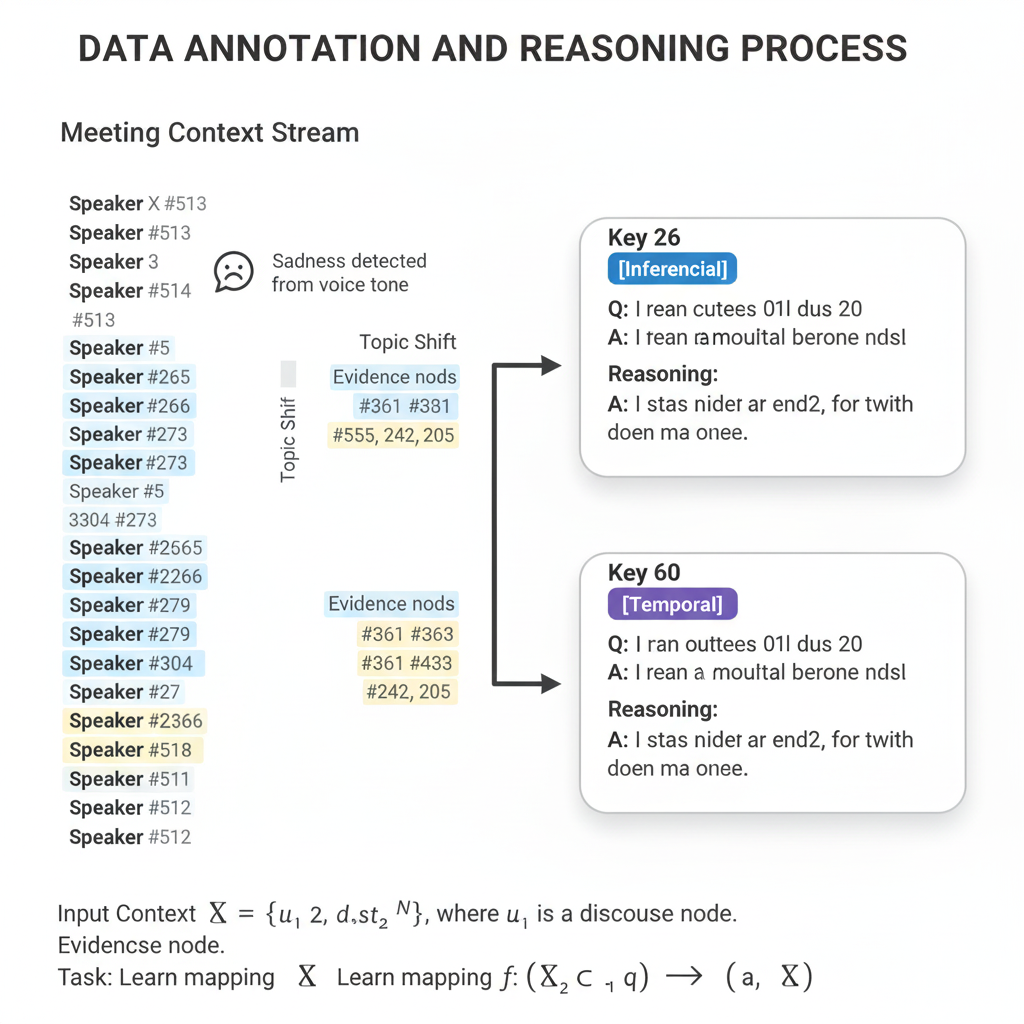
\includegraphics[width=1\linewidth]{figure/data_anno.png}
    \caption{Data annotation}
    \label{fig:data_anno}
\end{figure}

We propose a systematic pipeline to construct our dataset, ensuring both the structural complexity of the graph and the semantic richness of the QA pairs. The construction process consists of three phases: graph modeling, semi-automated question generation, and rigorous quality control.


\subsubsection{Evidence Extracting and Labeling}
To ensure balanced coverage of the five question categories, we employ specific strategies for each type:

\paragraph{Structure-Driven Generation (Factual, Temporal, Summarization).} 
We algorithmically sample specific subgraphs—such as a 30-minute time slice or a single speaker's full trajectory—and prompt SOTA LLM to generate questions grounded strictly within these scopes (e.g., \textit{``Summarize Speaker A's main argument''}).

\paragraph{Logic-Driven Generation (Inferential).} 
For multi-hop reasoning, we first identify discourse relations (e.g., causality, contrast) within the graph. We then extract the connected path (e.g., \textit{Issue} $\rightarrow$ \textit{Discussion} $\rightarrow$ \textit{Decision}) and prompt the LLM to construct questions that require traversing this path to answer.

\paragraph{Acoustic-Driven Generation (Acoustic-Aware).} 
To create questions involving paralinguistic features, we detect salient acoustic events (e.g., sudden volume spikes, laughter, or angry tone) in the waveform. These events serve as \textit{anchors}. We then prompt SOTA LLMs to craft cross-modal questions that link these acoustic cues to the semantic context (e.g., \textit{``Why did Speaker B raise their voice at this moment?''}).

Analysis of algorithms and time complexity can be found at Appendix \ref{alg:db_construction}.

\subsubsection{QA Schema and Evidence Grounding}
\label{sec:qa_schema}

To support long-form meeting question answering with explicit evidence grounding, we represent each QA example (Details can be found in Appendix \ref{qa_example}) as a structured record:
\begin{equation}
x = \langle k,\; \tau,\; q,\; a,\; \mathcal{E},\; r \rangle,
\end{equation}
where $k$ is a unique instance identifier, $\tau$ denotes the question type (e.g., \texttt{acoustic}), $q$ is the natural-language question, $a$ is the reference answer, $\mathcal{E}$ is a set of evidence pointers, and $r$ is an optional human-written reasoning note used for analysis.

We ground each answer on a minimal set of utterance nodes in our meeting graph $G=(V,E)$. Concretely, we define the utterance node set as $V_U \subset V$, and annotate evidence as:
\begin{equation}
\mathcal{E} = \{u_i\}_{i=1}^{m}, \quad u_i \in V_U,
\end{equation}
where each $u_i$ is uniquely indexed by its \texttt{utterance\_id}. In the released data format, \texttt{evidence\_nodes} is the list of such utterance IDs.

Each utterance node stores aligned multimodal attributes:
\begin{equation}
u = \langle id,\; spk,\; [t_s,t_e],\; text,\; audio\_ref \rangle,
\end{equation}
where $spk$ denotes the speaker label, $[t_s,t_e]$ is the absolute time span (in seconds) within the meeting, $text$ is the ASR transcript for the utterance, and $audio\_ref$ points to the corresponding audio interval (offsets in the original waveform or an external clip path). This design enables speaker-attributed and timestamped citations, as well as acoustic verification when the question type requires paralinguistic cues (e.g., surprise, laughter, emphasis).


We instruct annotators to select a \emph{minimal sufficient} evidence set $\mathcal{E}$ that fully supports the reference answer $a$. For \texttt{acoustic} questions, the selected utterance nodes must cover the time region where the relevant paralinguistic signal occurs, ensuring the answer can be verified against the raw audio via $audio\_ref$.